\documentclass[12pt]{article}
\usepackage{sydewkrpt}
\usepackage{longtable}
\usepackage{array}
\usepackage{ragged2e}
\usepackage{amsmath}
\usepackage{amssymb}
\usepackage{siunitx}

\usepackage{color}

\definecolor{mygreen}{rgb}{0,0.6,0}
\definecolor{mygray}{rgb}{0.5,0.5,0.5}
\definecolor{mymauve}{rgb}{0.58,0,0.82}

\usepackage{float}
\DeclareMathOperator*{\argmin}{\arg\!\min}
\DeclareMathOperator*{\argmax}{\arg\!\max}
\newcolumntype{P}[1]{>{\RaggedRight\hspace{0pt}}p{#1}}

\renewcommand{\thesection}{\arabic{section}}

%%%%%%%%%%%%%%%%%%%%%%%%%%%%
%%%    Begin Document    %%%
%%%%%%%%%%%%%%%%%%%%%%%%%%%%
\begin{document}
\pagenumbering{roman}

\waterlootitle{SYDE 531: Final Project Report}{
  Betting Strategies for an NCAA March Madness Tournament Bracket Using Dynamic Modern Portfolio Optimization\\
}{
  Brian Sinclair -- 20346309\\
  Riley Donelson -- 20342815\\
  }

\dotableofcontents

\newpage
\doublespacing
\pagenumbering{arabic}
\section{Introduction}
\setlength{\parindent}{1cm}
\subsection{Background}
This report details the design optimization of betting strategies for the NCAA Men's Division 1 Basketball Championship, commonly referred to as the ``March Madness'' tournament.
This tournament is a yearly event comprising of the top 64 teams in US College Basketball \cite{doi:10.1080/00031305.1996.10473540}.
It is structured in a classical tournament bracket format, beginning with 32 games (64 teams) and ending with one final Championship game.
The losing team from each game is eliminated from the tournament at each round, which cuts the number of games at each successive round in half.
This provides a tournament layout consisting of 6 rounds.

The attempt at predicting and/or betting on the games in this tournament is a common activity for many fans and followers of the sport.
In order to provide more informed decisions, the design optimization of betting strategies under probabilistic uncertainty was conducted using a modern portfolio theory mean-variance approach, combined with dynamic programming to select the optimal traversal of bet placements through the tournament.
The formulation of each optimization algorithm is provided, as well as the results and analysis of the solution.
Discussions on the results, sensitivity of the system, and conclusions are also provided. 

\subsection{Problem Definition}


\newpage
\section{Optimization Algorithms}
\subsection{Modern Portfolio Optimization}
\subsubsection{Approach Background}
As previously mentioned the goal of the project is to maximize the return on investment when betting on individual games in the yearly NCAA March Madness Tournament.
It was recognized early on that gambling in sports follows a similar behaviour to that of portfolio optimization between two assets. 
Any one game can be thought of as a portfolio where each asset is team A, or team B in the match-up.
The objective of any one game (as a portfolio) is to maximize return on investment when given a budget to spend on that game.
For the purposes of the tournament, instead of the portfolio being an individual game, it becomes an individual round (ie. Portfolio's 1 through 6 are Rounds 1 through 6).
The portfolio then changes from being constructed of assets as teams, to assets as each game.
In other words, one game is one asset in the portfolio (Round).
This outlook would follow a myopic outlook on Portfolio Theory for each round.
In the first round there is then 32 assets to purchase, 16 in the second, 8 in the third, and so on.

The bettor, or owner of this newly defined portfolio then has the option to buy into a game (wager a percentage of their budget) on either team A, or team B in an (A,B) match-up. 
If the wager is a positive value, then the bettor is placing a wager on team A.
If it is negative, then the bettor is placing a wager on team B.
The myopic optimization problem is to maximize the return on investment in any one round by maximizing budget allocation across all assets. 
The following section will aim to describe a novel application of expanding on the myopic approach into a dynamic portfolio optimization problem where the budget for the following round is the return on investment from the previous round.


\subsubsection{Setup}
Much of the general setup and background was already described. 
As previously mentioned the objective is to use modern portfolio theory techniques to determine a maximum return on investment for an individual round basis.
This is done using a mean-variance optimization approach described below.

\begin{equation}
\begin{aligned}
& \underset{x}{\text{max}}
& & f(x) =  E(R^Tx)-\theta\sqrt{var(R^Tx)}\\
& \text{s.t.}
& & \sum{x}=b\\
&&& |x_i| \leq b, \; i = 1, \ldots, m.
\end{aligned}
\label{portOpt}
\end{equation}
where,

\begin{table}[htbp!]
\begin{centering}
    \begin{tabular}{r l}
    $x_i:$      & Quantity wagered on a single game \\ 
    $R:$        & Vector of expected returns        \\ 
    $b:$        & Budget for any one round       	\\ 
    $m:$        & Total Number of games(assets)    	\\ 
    $\theta$	& Risk weighting					\\
    \end{tabular}
    \label{mop_vars}
    \caption{Variables used in the Mean-Variance Portfolio Optimization.}
\end{centering}
\end{table}
An important variable is the risk weighting variable $\theta$.
This signifies how important it is to account for risk in the optimization.
A low value here tells the algorithm to take a lot of risk in the wager, because risk is not important.
A high value will do the opposite and will make more conservative wagers between games in a round.

\subsubsection*{Stochastic Variables}
The objective is to maximize return while minimizing risk in the mean-variance approach, where return is the expected return based off of the stochastic return, and the risk is the variance.
Calculations for each is shown below:

\begin{equation}
\mu = E(R^Tx)=\sum r_i x_i
\end{equation}
\begin{equation}
var(R^Tx)=\sum x_i^2var(r_i)=\sum x_i^2(p_i(r_i-\mu)^2)
\end{equation}

\begin{equation*}
r_i=\frac{1}{p_i}x_i
\end{equation*}
where,

\begin{table}[htbp!]
\begin{centering}
    \begin{tabular}{r l}
    $r_i:$      & Expected return for one game \\ 
    $p_i:$      & Probability of team A or B winning the game \\ 
    \end{tabular}
    \label{op_vars}
    \caption{Stochastic Variables}
\end{centering}
\end{table}

To calculate the probability of each team winning a single game in a given round, a simple model is used.
The model uses the ordinal rankings given to each team by the NCAA committee and is calculated as follows with two teams A and B, in a given match-up.
\begin{equation}
p_A = 1 - \frac{rank A}{rank A + rank B}
\end{equation}
This method can be used with a reasonable confidence from the assumption that the NCAA committee uses a statistical method called the Ranking Percentage Index (RPI) to calculate their ordinal rankings.
RPI is a metric calculated from the weighted sum of three statistics: winning percentage, opponents' winning percentage, and opponents' opponents' winning percentage. 
This is the current standard for ranking teams 1 through 16 for each region (four regions: East, West, South, MidWest), creating the 64 teams that make-up the tournament.

\subsubsection{Assumptions}
One important assumption previously mentioned is that the rankings give a realistic probability of outcome.
However, this is very basic and more advanced statistical models would provide more accurate expected returns from any match-up.
Improvements to statistical modelling are described in conclusions and recommendations.

Additionally, in order to calculate the expected return the assumption of uniformity in distribution must be made for the stochastic variables.

\subsection{Dynamic Programming}
The method of discrete dynamic programming was employed in this solution to take the values provided from the mean-variance approach to portfolio optimization, and select the best ``path'' through the tournament where bets should be placed to maximize return.
The betting possibilities are discretized into 5 states, wherein one may utilize 100\%, 75\%, 50\%, 25\%, or 0\% of their budget on a round of the tournament.

Using the discrete dynamic programming methodology outlined in class, the problem was divided into stages, with each stage representing a round of the tournament.
This method depends on Bellman's principle of optimality, stated as follows:
\begin{quote}
\emph{``The optimal set of decisions in a multistage process has the property that whatever the initial stage, state and decisions are, the remaining decisions, given the current stage, must form a set of optimal decisions for the remaining problem.''}
\end{quote}
This gives rise to the recursive nature of the problem formulation.
A breakdown of the variables used in the analysis, and their meaning, is provided in Table \ref{dp_vars}. \\

\begin{table}[htbp!]
\begin{centering}
    \begin{tabular}{|l|l|}
    \hline
    Variable & Meaning           \\ \hline
    $x_{t}$        & Decision Variable \\ \hline
    $s_{t}$        & State Variable    \\ \hline
    $t$        & Stage Number             \\ \hline
    $f$        & Return            \\ \hline
    $f^{*}$       & Maximum Return    \\ \hline
    \end{tabular}
    \label{dp_vars}
    \caption{Variables used in the Dynamic Programming formulation.}
\end{centering}
\end{table}

A decision (the value of $x_{t}$) is required at each stage, where $t$ is the stage, and 1 $\le t \le$ 6.
Each stage has a state variable, $s_{t}$, and this state is divided into five states, one for each allowed percentage of the total budget to be bet.
At each stage (i.e. each round in the tournament), the dynamic programming system moves from the current state in the current stage to another ideal feasible state in the next stage.
This discrete dynamic programming methodology is able to solve each stage problem individually by considering the return function for the current stage, and the optimal function, $f^{*}$, from the next stage ($t + 1$) to the end of the horizon (6 rounds).
In order to accomplish this, a recursive equation was constructed, as shown in Equation \ref{dp_recursive}.

\begin{equation}
f_{t}(s_{t}(i)) = \max \ [r_{t}(x_{t},s_{t}(i)) + f^{*}_{t+1}(s_{t+1}(j))]
\label{dp_recursive}
\end{equation}

This way, the system is able to determine optimal decisions for the problem overall, from any given state.
The full list of decisions and their individual returns are available at the end of the procedure.

Upon formulation of the problem, the dynamic programming portion of the system was then implemented in Matlab to generate solutions, given inputs from the prior mean-variance method.
The full implementation is given in Appendix A.
The data from the mean-variance solution was structured into a 5x5x6 3-dimensional matrix, where each row represents the returns of each state transition to the next stage.
Each ``page'' of this matrix (i.e. along the 3rd dimension) represents the data for each stage, or round, of the tournament.
With the data modelled appropriately, the optimal return (and its location) for the final round of the tournament was found and placed into a list holding each of the optimal decisions throughout the tournament.
Then, each stage of the tournament was looped through in a backwards fashion, and the optimal path of bets through the tournament was generated recursively.
The returns from each stage are then summed, to provide a look at the total optimal return for the tournament.

\subsubsection{Assumptions}
One assumption that needs to be made in calculating and implementing a dynamic programming graph traversal is that probabilities of future rounds do not change.
The algorithm finds an optimal path of discretized wagers progressing through the six rounds of the tournament. 
All benefits from from one round to another are calculated based off of expected return in the following round.
In order to calculate expected return, match-ups for all rounds of the tournament would need to be known, and correspondingly, the odds of each team is all match-ups. 
For the purposes of this project, match-ups from a past tournament was used to have knowledge of these match-ups, however this would not be realistic.
However this does allow for accurate knowledge of probabilities of every match-up in all rounds of the tournament and is necessary for implementing dynamic programming.

This could be overcome by using an intelligent system to predict probabilities of future match-ups and dynamically change algorithm as tournament progresses. 
For example, if round 1 of the tournament is complete and teams in round 2 were not predicted correctly then would need to dynamically change betting towards teams in current round (round 2).
The machine learning algorithm would then adopt a new prediction for rounds 3 through 6 and the entire betting path would change.
One solution to an intelligent system would be to implement an artificial neural network to use backpropagation techniques from past data to predict the outcome of a tournament. 
The team is working on this out of interest but it is not discussed further in this report.

\section{Results and Analysis}
\subsection{Modern Portfolio Optimization}
With a starting budget of "1" in \eqref{portOpt}, the budget dynamically changes based off the return from the previous round and the budget not yet used.
The new budget is calculated as follows:
\begin{equation*}
currBudget = currPercent*(prevRtn + (1-prevPercent))
\end{equation*}
The maximization is then calculated again for the current round using the formulation defined in \eqref{portOpt} with the new portfolio of games to wager towards.
The algorithm calculates the expected return given the risk associated with it for each discretized percent allocation cascading through the 6 rounds.
The result is formulating the recursive benefit transitioning between stages in the Dynamic Programming problem.

After obtaining an optimal wager between games in a single round (or stage), the algorithm checks if the team that was wagered towards won in that round to obtain the return for a given game.
In other words, if 20\% of the budget was spent on a team A in an (A,B) match-up the wager would be positive.
The algorithm them would check if team A won, before getting its return.
If team B won the match, then a return of zero would result from that game.
This is verified for all games in a round and summed to get the entire return.

To implement the optimization, the $fmincon$ function in Matlab was used with the $"active-set"$ algorithm.
The code and setup is found in Appendix A.

\subsection{Sample Inputs, Outputs, and Detailed Solution}
A sample of the the dynamic programming formulation is shown in Figure \ref{sampleDP}.
The graph shows the optimal path and returns calculated for each transition from the mean-variance portfolio optimization algorithm.
The portfolio optimization uses the recursive function defined in \eqref{dp_recursive} to calculated the benefit of transitioning between rounds.
As previously mentioned, the goal of the Dynamic Programming formulation is to find the optimal path shown in Figure \ref{sampleDP}.
\begin{figure}[H]
\centering
	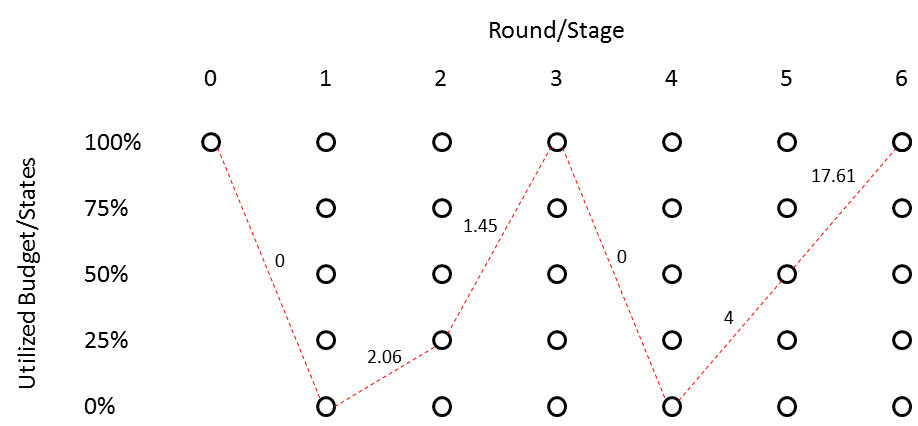
\includegraphics[scale=.5]{sampleDP.png}%
	\caption{Sample Path in Dynamic Programming Formulation}
	\label{sampleDP}
\end{figure}
Round 0 is shown in the formulation to signify that the budget before entering into the tournament starting at 100\%.
It's determined that it is more beneficial to not spend any of the budget in the first round and then traversing through, and eventually spending all of the budget in the sixth round.

\subsection{Sensitivity Analysis}
\subsubsection{Risk}
As previously mentioned, the risk is weighted by a factor of $\theta$ in \eqref{portOpt}.
Because the calculated probability follows a simple model that is not really representative of the actual probability of a team winning, the risk calculation from variance is also not representative of real risk associated with the bet made. 
With varying risk weight $\theta$, the optimal asset allocation should change. 
It was determined that early on in the tournament, a change in risk seems to have an expected change in outcome of wager allocation.
For example, telling the algorithm to weight risk low (take a lot of risk) in a game where a team ranked 1 is playing a team ranked 16, the algorithm often places a wager on team 16 -- as expected.
However, as the tournament progresses, the bettor is unable to weight risk low enough for the algorithm to gamble on the team with a lower probability.
This is because there are less teams and therefore less variance.

One way to overcome this is to follow the idea of taking less risk early on in the tournament and more as it progresses.
This is done by multiplying $\theta$ by the number of teams in a round -- so that early on risk matters more than later in the tournament because $\theta$ is a greater value in round 1.
After many values of $\theta$ where attempted it was determined that a value of "1" resulted in the best outcome.

\subsubsection{Initial Guess}
Another sensitive component to using the $"acive-set"$ algorithm in $fmincon$ was the initial guess -- especially for rounds where there are not many games (ie. Round 6 only has one game).
The algorithm tends to find a local maximum biased towards the initial guess.
In other words, if the initial guess was positive (a bet would be placed on team A in an (A,B) match-up), then the algorithm would also find a positive solution -- no matter how much risk is varied as previously discussed).

\subsection{Inferences on Problem Solutions}

\newpage
\section{Recommendations \& Conclusions}
\subsection{Probability Model}

\subsection{Two Stage Stochastic Optimization}

\subsection{Intelligent Tournament Forecasting}

\newpage
\section{References}
\bibliographystyle{IEEEtran}
\bibliography{bib}

\newpage
\section{Appendix A: Full Implementation}
\subsection{Dynamic Programming}
\begin{verbatim}
clear;

num_stages = 6;	% number of rounds in the tournament
num_states = 5;	% number of possible bets at each round

opt_list = [];	% stores optimal return and location of bet
[state_benefit, opt_dsg] = max(benefits(:, :, num_stages));
[row, col] = max(state_benefit);
state_benefit = row;
opt_dsg = opt_dsg(col);

opt_list = [opt_list; state_benefit, opt_dsg];

for curr_stage = (num_stages-1):-1:1
	[state_benefit, opt_dsg] = max(benefits(:, opt_dsg, curr_stage));
	opt_list = [opt_list; state_benefit, opt_dsg];
end

opt_list
\end{verbatim}

\begingroup
    \fontsize{8pt}{10pt}
    \spacing{1}
    \lstset{breaklines=true}
	\definecolor{mygreen}{rgb}{0,0.6,0}
	\definecolor{mygray}{rgb}{0.5,0.5,0.5}
	\definecolor{mymauve}{rgb}{0.58,0,0.82}
	
	\lstset{ %
	  backgroundcolor=\color{white},   % choose the background color; you must add \usepackage{color} or \usepackage{xcolor}
	  basicstyle=\footnotesize,        % the size of the fonts that are used for the code
	  breakatwhitespace=false,         % sets if automatic breaks should only happen at whitespace
	  breaklines=true,                 % sets automatic line breaking
	  captionpos=b,                    % sets the caption-position to bottom
	  commentstyle=\color{mygreen},    % comment style
	  deletekeywords={...},            % if you want to delete keywords from the given language
	  escapeinside={\%*}{*)},          % if you want to add LaTeX within your code
	  extendedchars=true,              % lets you use non-ASCII characters; for 8-bits encodings only, does not work with UTF-8
	  frame=single,                    % adds a frame around the code
	  keepspaces=true,                 % keeps spaces in text, useful for keeping indentation of code (possibly needs columns=flexible)
	  keywordstyle=\color{blue},       % keyword style
	  language=Octave,                 % the language of the code
	  morekeywords={*,...},            % if you want to add more keywords to the set
	  numbers=left,                    % where to put the line-numbers; possible values are (none, left, right)
	  numbersep=5pt,                   % how far the line-numbers are from the code
	  numberstyle=\tiny\color{mygray}, % the style that is used for the line-numbers
	  rulecolor=\color{black},         % if not set, the frame-color may be changed on line-breaks within not-black text (e.g. comments (green here))
	  showspaces=false,                % show spaces everywhere adding particular underscores; it overrides 'showstringspaces'
	  showstringspaces=false,          % underline spaces within strings only
	  showtabs=false,                  % show tabs within strings adding particular underscores
	  stepnumber=2,                    % the step between two line-numbers. If it's 1, each line will be numbered
	  stringstyle=\color{mymauve},     % string literal style
	  tabsize=2,                       % sets default tabsize to 2 spaces
	  title=\lstname                   % show the filename of files included with \lstinputlisting; also try caption instead of title
}
\subsection{Mean-Variance Portfolio Optimization}
\lstinputlisting[language=Matlab]{betOpt_marchmadness.m}

\subsubsection{Mean-Variance Objective Function}
\lstinputlisting[language=Matlab]{mean_var_func.m}

\subsubsection{Constraints}
\lstinputlisting[language=Matlab]{absSum.m}

\subsubsection{Verify Winners}
\lstinputlisting[language=Matlab]{checkwinners.m}

\subsubsection{Dynamic Programming Setup}
\lstinputlisting[language=Matlab]{DPsetup.m}

\end{document}